\chapter{Methodology}

\section{Problem description}
Most of the problem description is taken from the \emph{DISPLIB format specification} \cite{kloster2025displibspec}, a concise explanation is in accompanied paper \cite{kloster2025displiblibrarytraindispatching}.

Each instance in the \emph{DISPLIB} library consist of set of trains and an objective to be minimized. All data is presented in JSON format \cite{pezoa2016foundations}. Train is defined by an operation graph which is DAG, operation has the following content:

\begin{itemize}
    \item minimal duration
    \item start lower bound (optional)
    \item start upper bound (optional)
    \item list of successors
    \item list of required resources
    \begin{itemize}
        \item resource name
        \item release time
    \end{itemize}
\end{itemize}    

Data \ref{data:op} show and example of an operation entry in the instance JSON.

All operation graphs have one entry (start) operation, with no predecessors, and one exit (end) operation, with no successors. Each operation ends exactly when the successor operation starts, exit operation has no end. 

Resources are anything that is required by the operation, typically physical sections of the railway network. Resources can only be used by one operation at the time and are released after the end of the operation that uses it plus the defined release time.

Objective is defined by a list of objectives components, each with the following content 

\begin{itemize}
    \item train
    \item operation
    \item threshold
    \item coefficient (linear objective)
    \item increment (stepwise objective)
\end{itemize}

\begin{remark}
While the format allows both coefficient and increment to be non-zero, in practice none of the instances mix both in one objective component.
\end{remark}

Data \ref{data:obj} show and example of an objective component entry in the instance JSON.

The total objective $J$ is defined as a sum of components for active operations only,

\begin{equation}
J = \sum_{o \in O_{a,J}} c_o \max\{0, t_o - \bar{t}_o\} + d_o H(t_o - \bar{t}_o),
\end{equation}

where $O_{a,J}$ is a set of active operations that have an objective component, $t_o$ is start of the operation, $\bar{t}_o$ is the threshold for the operation, $c_o$ is the linear objective coefficient, $d_o$ is the stepwise objective increment, and $H(\cdot)$ is Heaviside step function \cite{abramowitz1972handbook}.

A solution to the problem is a sequence of events, each event entry corresponds to start of an operation and contains:
\begin{itemize}
    \item train
    \item operation
    \item time
\end{itemize}

Solution is also presented in a JSON format, data \ref{data:events} shows truncated solution example. To reiterate, the end event of an operation is the start event of its successor.

\begin{displaycquote}[Feasible solution requirements in \emph{DISPLIB} format specification]{kloster2025displibspec}
    \begin{itemize}
        \item The sequence of events is given in chronological order, i.e., the time of each event is greater than or equal to the time of all preceding events.
        \item The subsequence of operations applying to each train forms a path through that train’s operations graph, starting at the entry operation and ending at the exit operation.
        \item The time value of each start event satisfies the lower and upper bounds on the start time of the operation.
        \item The duration from each start event to the corresponding end event must be greater than or equal to the minimum duration of the corresponding operation.
    \item For any pair of operations $o_1$ and $o_2$, where:
        \begin{itemize}
            \item the start event of $o_1$ precedes the start event of $o_2$ in the global sequence, and $o_1$ and $o_2$ belong to different trains, and
            \item $o_1$ and $o_2$ use a common resource $r$,
        \end{itemize}
        the following must hold:
        \begin{itemize}
            \item the end event for $o_1$ precedes the start event for $o_2$ in the global sequence, and
            \item the duration from the end event of $o_1$ to the start event of $o_2$ is greater than or equal to the release time of resource $r$ in $o_1$.
        \end{itemize}
    \end{itemize}
\end{displaycquote}

While the events in the solution have a time, their order in the list is still significant, as they define in which order the resources are unlocked and locked. This is to prevent a resource swap situation described in section \ref{sec:swap}.

\subsection{Example problem}
To illustrate the format we have prepared example problem, the railway network diagram is in picture \ref{fig:railway_example}. The network consists of 3 trains, 18 operations, and 8 railway sections, corresponding to resources.

\begin{figure}[htbp!]
\caption{Example railway network}
\label{fig:railway_example}
\begin{center}
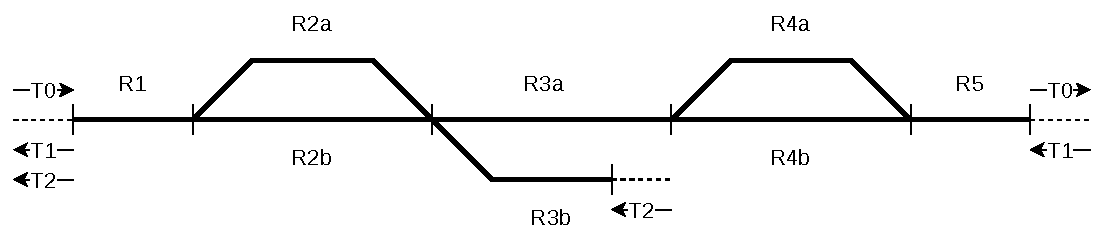
\includegraphics[width=\textwidth]{img/displib_example.pdf}
\end{center}
\end{figure}


The corresponding operation graph for train 0 (first) is in figure \ref{fig:train_dag}, JSON entry for operation 4 is in data \ref{data:op}, and JSON entry for objective component for the last operation is in data \ref{data:obj}.

\begin{figure}[htbp!]
\caption{Operation graph for train 0}
\label{fig:train_dag}
\begin{center}
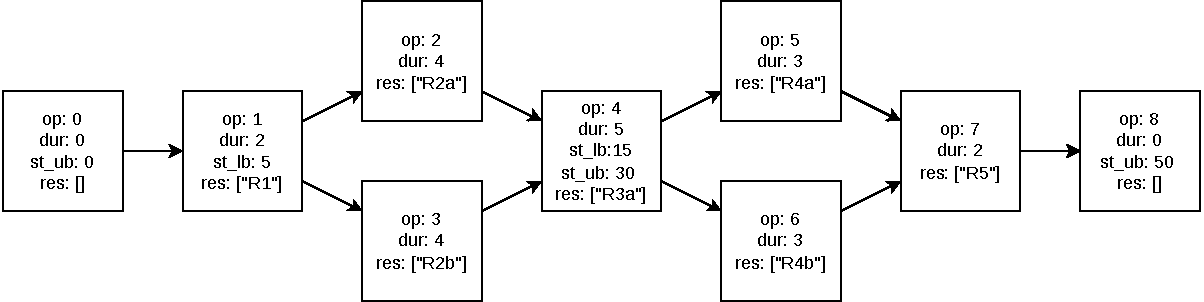
\includegraphics[width=\textwidth]{img/train_dag.pdf}
\end{center}
\end{figure}

\begin{data}[float, caption={JSON operation entry}, label=data:op]
{
    "start_lb": 0,
    "start_ub": 50,
    "min_duration": 5,
    "resources": [
        {
            "resource": "R3a",
            "release_time": 0
        }
    ],
    "successors": [
        5,
        6
    ]
}
\end{data}
\begin{data}[float, caption={JSON objective component entry}, label=data:obj]
{
    "type": "op_delay",
    "train": 0,
    "operation": 8,
    "threshold": 25,
    "coefficient": 1
}
\end{data}

\begin{data}[float, caption={JSON solution truncated}, label=data:events]
{
    "events": [
        ...,
        {
            "train": 0,
            "operation": 5,
            "time": 15
        },
        {
            "train": 1,
            "operation": 4,
            "time": 15
        },
        ...
    ],
    "objective_value": 25
}
\end{data}


\FloatBarrier

\subsection{Resource swap}
\label{sec:swap}

Consider the situation as in figure \ref{fig:swap_railway}, where 2 trains A and B are passing a section of 2 resources X and Y in opposite direction. If we were to set events A2 and B2 to the same time, we would not have a resource collision on either resources (overlap of intervals for operations A1 and B2 on resource X or A2 and B1 on resources Y) but in reality the trains would collide. 

\begin{figure}[htbp!]
\caption{Resource swap railway}
\label{fig:swap_railway}
\begin{center}
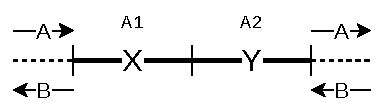
\includegraphics[width=.5\textwidth]{img/swap_railway.pdf}
\end{center}
\end{figure}

In this situation, resource Y is being acquired by A while holding X and X is being required by B while holding Y.

We can detect the resource swaps using an event graph by cycle detection, like in figure \ref{fig:swap_event} where A2 and B2 form a cycle.

\begin{figure}[htbp!]
\caption{Resource swap event graph}
\label{fig:swap_event}
\begin{center}
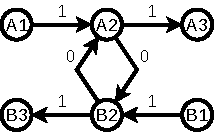
\includegraphics[width=.5\textwidth]{img/swap_event_graph.pdf}
\end{center}
\end{figure}

\begin{remark}
Using cycles in event graph to detect resource swaps only works if all resource precedence edges are present, otherwise we still might have a resource swap situation because the current event times do not create a collision and one or both of the edges that would create the cycle in the event graph are missing.
\end{remark}


